\section{Cached design}

\begin{frame}{Requirements}

	Design goals for cached:
	\begin{itemize}
		\item Create something close to the Archipelago logic
		\item Measure the best possible performance we can get
	\end{itemize}

	\note{Επιλέξαμε λοιπόν να δημιουργήσαμε τη δική μας λύση. Την ονομάσαμε 
		cached από το cache daemon}
	\note{Ορίσαμε τους εξής γενικούς στόχους:
		\begin{itemize}
			\item Να είναι κοντά στη λογική του Archipelago
			\item Η υλοποίηση να είναι όσο το δυνατόν πιο γρήγορη 
				για να δουμε αν μια Αρχιπελαγική λύση μας 
				βοηθάει
		\end{itemize}
	}
	\dspc
	Stricter requirements for cached:
	\begin{itemize}
		\item Nativity
		\item Pluggability
		\item In-memory
		\item Low indexing overhead
	\end{itemize}
	\note{Ακόμα, θέσαμε κάποιες πιο αυστηρές απαιτήσεις για την υλοποίηση 
		μας: 1)να είναι peer του Archipelago, 2) να μπορεί να ενεργοποιείται 
		και να απενεργοποιείται σε ένα σύστημα που είναι εν λειτουργία, 3)να 
		χρησιμοποιεί τη RAM, 4)ο indexing μηχανισμός να είναι γρήγορος}
\end{frame}

\begin{frame}{Cached design}
	\note{Εδώ βλέπουμε το design του cached. Ο cached μπαίνει ανάμεσα στον vlmc 
		και στον blocker και cach-άρει ότι άιτημα για αντικείμενα πάει στο 
		storage}
	\note{Οι εργασίες του cached χωρίζονται σε 5 κατηγορίες:}
	\note[item]{Στην διαχείριση των αιτημάτων από και προς vlmc, blocker}
	\note[item]{Στο indexing (εύρεση και καταχώρηση) των αντικειμένων}
	\note[item]{Στην υπο συνθήκες εκτέλεση εργασιών}
	\note[item]{Στην ασφαλή μετάδοση των cachαρισμένων δεδομένων στο 
		storage}
	\note[item]{Καθώς επίσης και στην ασφαλή επεξεργασία των cachαρισμένων 
		δεδομένων}
	\note[item]{\click}

	\begin{columns}[T]
		\begin{column}{0.65\textwidth}
			\includegraphics<1>[width=\columnwidth]{images/cached-design2.pdf}
			\includegraphics<2>[width=\columnwidth]{images/cached-design-comp2.pdf}
		\end{column}
		\begin{column}{0.35\textwidth}
			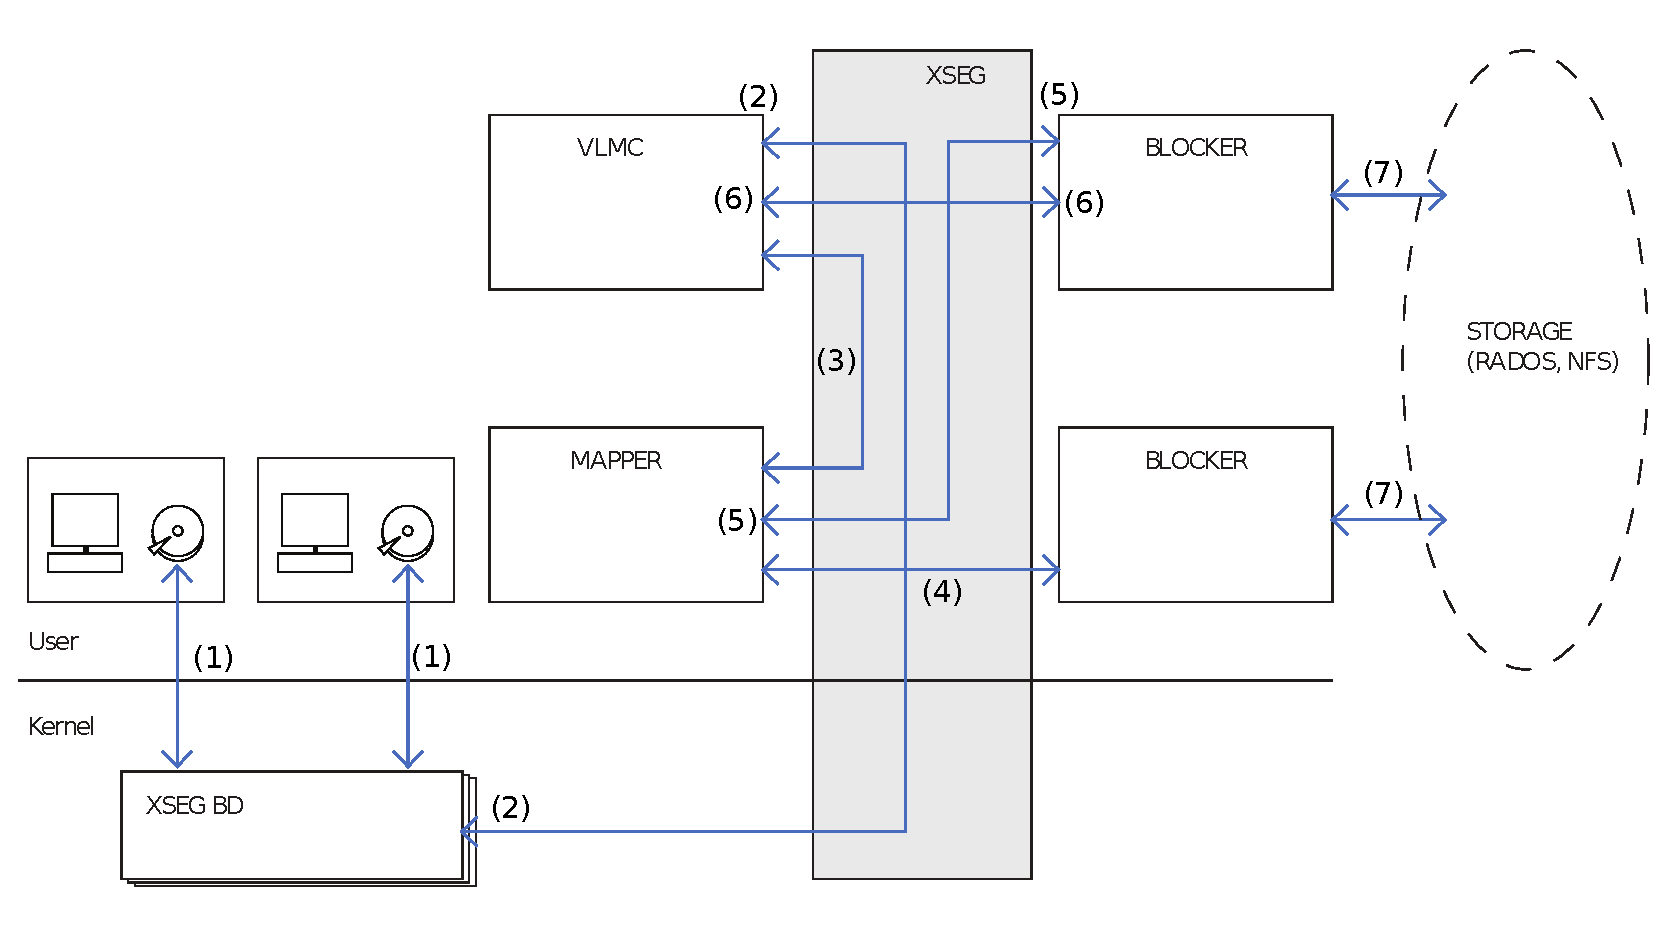
\includegraphics[width=\columnwidth]{images/new_sxima_numbered.pdf}
		\end{column}
	\end{columns}
	\note[item]{Και εδώ βλέπουμε τα διακριτά κομμάτια κώδικα που υλοιποιούν τα 
		παραπάνω και τα οποία θα συζητήσουμε ευθύς αμέσως}
\end{frame}

\begin{frame}{Xcache design}
	\centering\includegraphics<1>[height=0.6\textheight]{images/xcache-design.pdf}
	\centering\includegraphics<2>[width=\textwidth]{images/xcache-entry.pdf}

	Xcache is responsible for: 1) entry indexing, 2) entry eviction, 3) 
	concurrency control

	\note[item]{Αυτό είναι το xcache, που είναι υπεύθυνο για την
		\begin{itemize}
			\item Indexing των αντικειμένων
			\item Eviction αντικειμένων από την cache με τη χρήση LRU
			\item Χειρισμό προσβάσεων από πολλαπλά threads
		\end{itemize}
	}
	\note[item]{Έχουμε δυο hash table, το καθένα με το δικό του lock, ένα χώρο 
		που αποθηκεύονται οι εγγραφές των αντικειμένων και μόνο (όχι τα 
		δεδομένα, προσοχή) και μια στοίβα όπου κρατιούνται indexes των 
		ελεύθερων entries, προστατευόμενη από ένα lock.}
	\note[item]{To ένα hash table <αυτό> που κρατάει τα ονόματα των cached 
		αντικειμένων.}
	\note[item]{To άλλο hash table κρατάει τα ονόματα των evicted αντικειμένων 
		έως ότου ελευθερωθούν ή ξαναγίνουν cached.}
	\note[item]{Ο αποθηκευτικός τους χώρος είναι preallocated και είναι <αυτό>.  
		Σε αυτό το χώρο, η αναφορά γίνεται με δείκτες.}
	\note[item]{Τα ελεύθερα entries είναι στη στοίβα αυτή.}
	\note[item]{\click}
	\note[item]{Κάθε item έχει ένα reference counter για να ξέρουμε πόσοι το 
		χρησιμοποιούν, όνομα, και δείκτες για την lru}
	\note[item]{Συγκεκριμένα, στο παράδειγμα αυτό, το entry αυτό είναι το 
		τελευταίο LRU, αυτό είναι το MRU κτλ. χέρι στον πίνακα}
	\end{frame}

\begin{frame}{Xworkq design}
	\centering\includegraphics<1>[width=\textwidth]{images/xworkq-design.pdf}

	Xworkq is responsible for concurrency control
	\note[item]{xworkq υπεύθυνο για την ασφαλή επεξεργασία των δεδομένων 
		ενός αντικείμενου.}
	\note[item]{Δεν μπορεί πάνω από ένας να πειράζει τα data ενός thread. Το 
		spinning είναι αργό, όλοι τοποθετούν μια δουλειά σε μια ΟΥΡΑ, ένας την 
		εκτελεί.  Έτσι, ένα thread εκτελεί μια δουλειά και τα υπόλοιπα είναι 
		ελεύθερα να κάνουν κάτι πιο χρήσιμο}
	\end{frame}

\begin{frame}{Xwaitq design}
	\centering\includegraphics<1>[width=\textwidth]{images/xwaitq-design.pdf}

	Xwaitq is responsible for deferred execution
	\note[item]{xwaitq υπεύθυνο για την υπό συνθήκη εκτελεση εργασιών}
	\note[item]{Αν π.χ. μας τελειώσει ο χώρος, δεν μπορούμε να περιμένουμε 
		σύγχρονα. To thread μπορεί να τοποθετήσει μια δουλειά και μετά 
		να εκτελέσει κάτι άλλο}
\end{frame}

\begin{frame}{Bucket pool}
	Cached divides an object (commonly 4MB) to buckets (commonly 4KB) which are 
	always fully written.
	When an object is indexed however, it does not have immediate access to all 
	of its buckets because:
	\begin{itemize}
		\item RAM is limited
		\item Most objects would probably be half-written
	\end{itemize}
	\note[item]{Σπάμε τα objects (τυπικά έχουν 4MB) σε buckets (τυπικά των 
		4KΒ).  Άρα κάθε object έχει 1024.}
		\note[item]{Το ότι κάνουμε index ένα object δε σημαίνει ότι αυτομάτως 
			έχει και τα 1024 buckets}
	\note[item]{Δεν υπάρχει τόση RAM και άλλωστε πολλά objects μπορεί να είναι 
		μισό-γραμμένα}
	Ideally, we want to:
	\begin{itemize}
		\item Decouple the objects from their data
		\item Cache unlimited objects but put a limit on their data
	\end{itemize}
	\note[item]{Ιδανικά θέλουμε να διαχωρίσουμε την καταχώρηση/όνομα του 
		αντικειμένου από τα δεδομένα του. Δυνητικά θα μπορούμε να καταχωρούμε 
		πάρα πολλά αντικείμενα αλλά θα έχουμε μικρότερο cache size}

	Solution:
	\begin{itemize}
		\item Preallocated data space (=cache size) separated in buckets
		\item Every object requests a range of buckets for a request
		\item When an object is evicted, its buckets are reclaimed
	\end{itemize}
	\note[item]{Preallocated χώρος, όλοι παίρνουν indexes από αυτό (Θυμίζει 
		xcache, ΠΕΣ για WAITQ}
\end{frame}

\begin{frame}{Other important cached tasks}

	Several other key-tasks are:
	\begin{itemize}
		\item Book-keeping
		\item Cache write policy
		\item Asynchronous task execution
		\item Data propagation
	\end{itemize}
	\note{Το cached είναι επίσης επιφορτισμένο και με άλλες δουλειές όπως:
		\begin{itemize}
			\item Κρατάει στατιστικά (πόσα entries είναι dirty, 
				πόσα buckets έχει κάνει allocate ένα entry
			\item Εφαρμόζει writeback/writethrough πολιτική
			\item Φρόντίζει ώστε οι εργασίες να μπορούν να γίνουν 
				ασύγχρονα
			\item Και φυσικά φροντίζει τα δεδομένα να γράφονται 
				σωστά στο storage
		\end{itemize}
	}
\end{frame}

\begin{frame}{Cached flow}
	\includegraphics<1>[height=0.8\textheight]{images/cached-design2.pdf}
	\includegraphics<2>[height=0.8\textheight]{images/cached-design-comp2.pdf}

	\note[item]{Εδώ παίζεις με τα slides}
	\note[item]{Θα παρουσιάσουμε πολύ γρήγορα τη ροή ενός αιτήματος στον 
		cached}
	\note[item]{Έρχεται request, το κάνουμε index, μπαίνουμε στη workq και 
		πειράζουμε τα δεδομένα του και ανάλογα το cache policy το 
		γράφουμε πίσω στον blocker αλλιώς τελειώσαμε}
	\note[item]{Optional σεναρια:
		\begin{itemize}
			\item Αν γίνει ένα eviction, πρέπει να γράψουμε τα 
				δεδομένα του πίσω με ασφάλεια. Επειδή το 
				αντικείμενο μπορει να καταχωρηθεί, να μπει και 
				να ξαναβγεί, πρέπει να είμαστε προσεκτικοί
			\item Αν ξεμείνουμε από πόρους (χώρο στο hash table, 
				buckets κτλ, πρέπει να συνεχίσουμε μονο όταν 
				μπορούμε
		\end{itemize}
	}
\end{frame}
